\chapter[Seapp documentation]{SEApp documentation}\label{appendix:seapp_analysis}

\begin{wrapfigure}{r}{0.3\textwidth}
	\begin{center}
          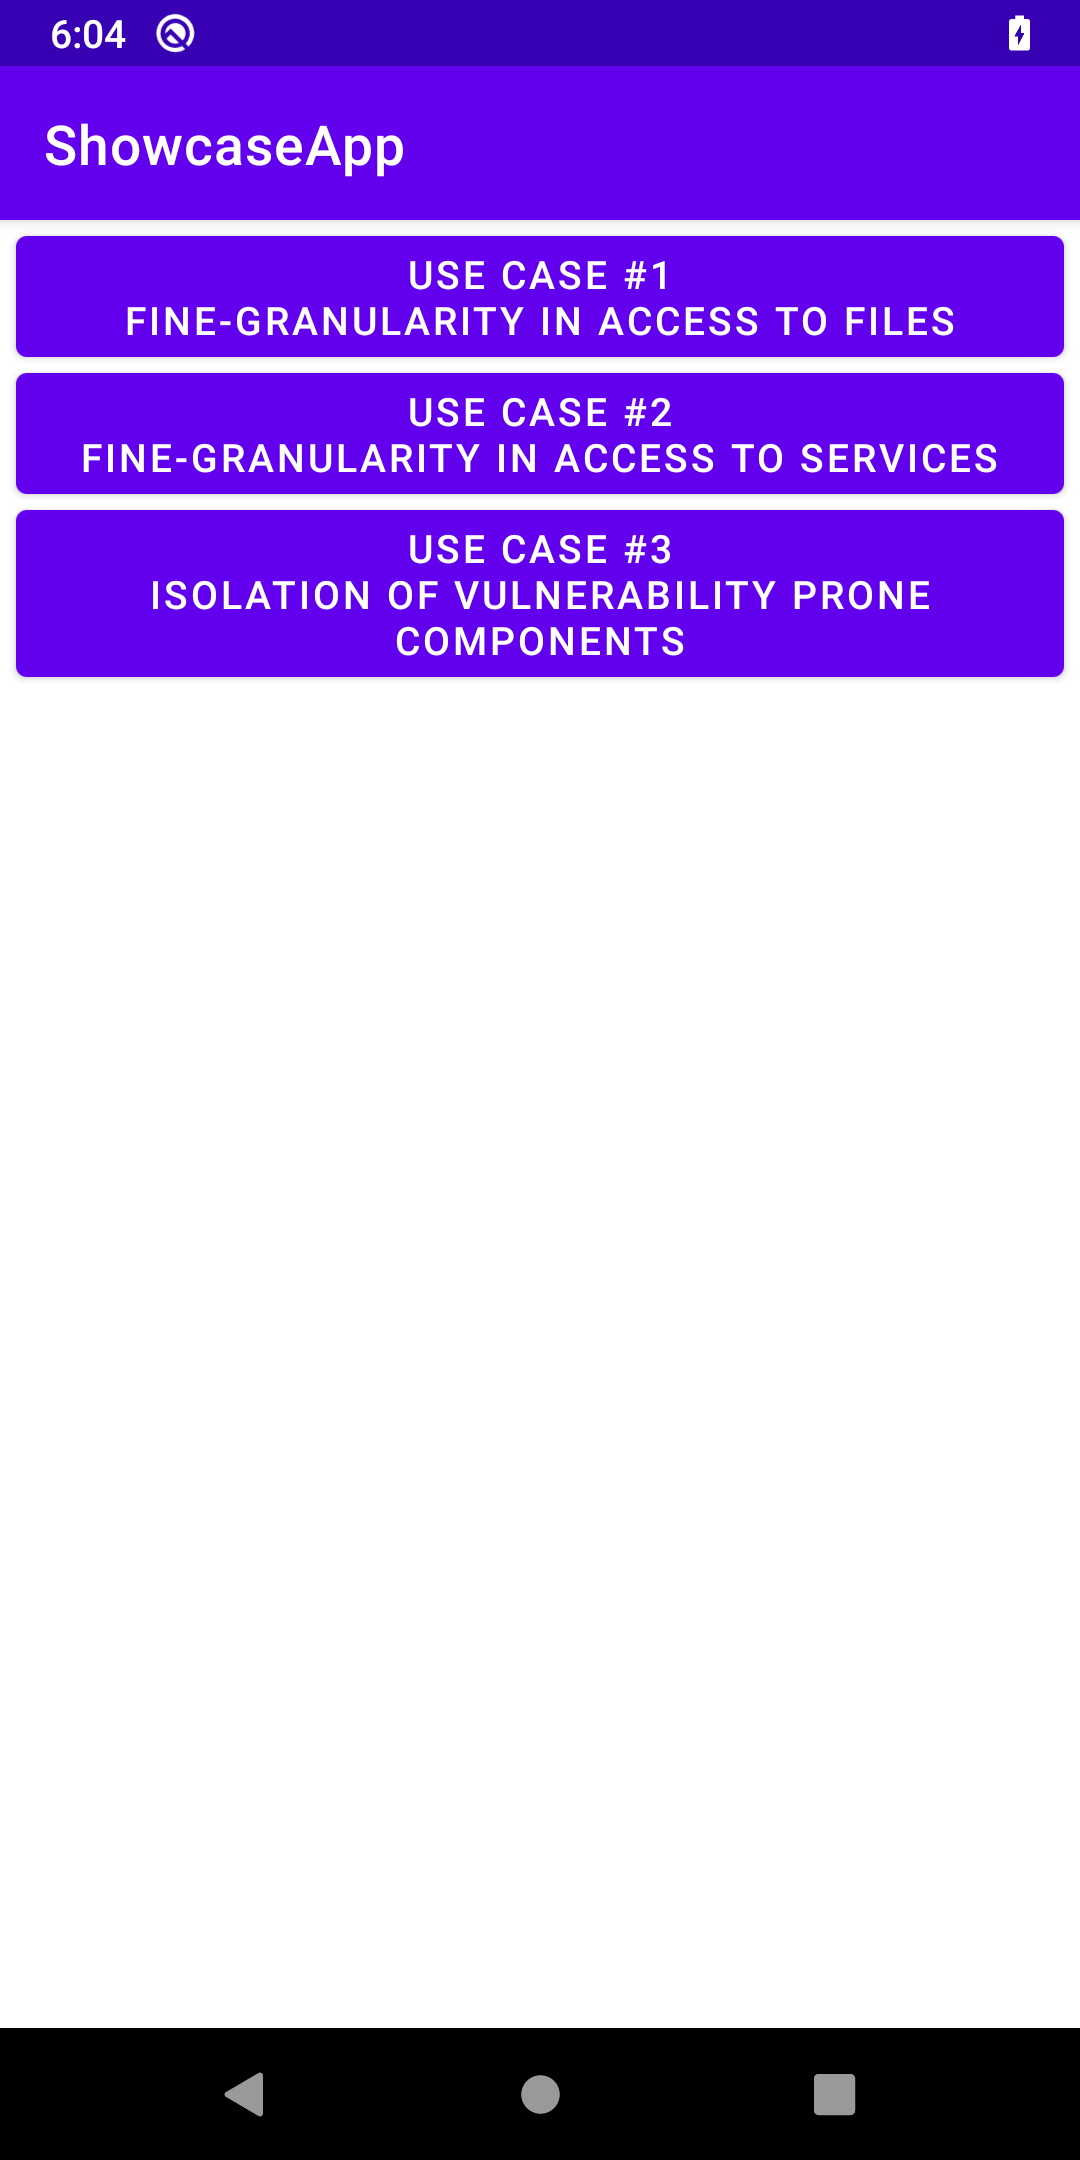
\includegraphics[width=0.28\textwidth]{chapters/seapp/figs/ae/MainActivity.png}
        \end{center}
	\caption{MainActivity}
	\label{fig:seapp_mainactivity_view}
      \end{wrapfigure}
      
This chapter gives a technical demonstration of the security measures
introduced by \seapp. The description is based on the showcase app
presented in Section~\ref{sect:seapp_motiv}. We show that: (1) the
showcase app can operate without a policy module; in this mode, its
vulnerabilities can be exploited; (2) the showcase app can also
operate with the policy module listed in
Appendix~\ref{appendix:seapp_policy} and use the services offered by
SEApp; in this mode, the internal vulnerabilities are no longer
exploitable.

The showcase app has a minimal structure. Its entry point is the {\em
  MainActivity} (Figure~\ref{fig:seapp_mainactivity_view}), which is associated with the {\em core\_logic}
process. From the {\em MainActivity} it is possible to send a {\em
  startActivity} intent to one among {\em UseCase1Activity}, {\em
  UseCase2Activity} and {\em UseCase3Activity}; the entry points of
use cases~1, 2 and~3, respectively. For each entry point {\em Zygote}
starts a dedicated process and, according to the content of the
\seappcontexts (in Listing~\ref{seapp_seappctxp}), assigns its
specific domain ({\tt user\_logic\_d} to UC\#1, {\tt ads\_d} to UC\#2,
{\tt media\_d} to UC\#3).  A dedicated description of each use case
follows.

\vspace{-1.6em}\section{Use case 1}\label{appendix:seapp_uc1}

\vspace*{-0.5em}
In this use case we demonstrate how an app could benefit from the
fine-granularity access to files.  In particular, we show how the {\em
  UseCase1Activity}, suffering of a path traversal vulnerability,
cannot be exploited when the app is associated with a properly
configured policy module.  According to the Google Play Protect report
on common application
vulnerabilities~\cite{seapp_common_play_protect_vulnerabilites},
unsanitized path names that lead to path traversal are a primary
source of problems in applications.

{\em UseCase1Activity} is quite simple: it displays the content of a
file given its relative path through an intent
(Figure~\ref{fig:seapp_uc1_views}a). While this may be fine when the
intent comes from trusted components, the activity supports also
implicit intents coming from untrusted sources. This makes the
vulnerability easily exploitable by an attacker targeting the
confidential files written by the {\em core\_logic} components.
%
In our setup phase, we leverage {\em MainActivity} to create an
internal directory structure by using the {\tt android.os.File}
abstraction, which sets file and directory context upon its creation
(see Section~\ref{sect:seapp_impl_files}). Two directories are
created: {\tt user/} and {\tt confidential/}; inside both folders a
file {\tt data} is saved.
%
To test this use case, we first start {\em UseCase1Activity}, then we
send an intent to ``confuse'' {\em UseCase1Activity} into showing us
the content of {\tt confidential/data}. This can be done via ADB with
the command:
\begin{lstlisting}[numbers=none]
adb shell am start
-n com.example.showcaseapp/.UseCase1Activity
-a "com.example.showcaseapp.intent.action.SHOW"
--es "com.example.showcaseapp.intent.extra.PATH" "../confidential/data"
\end{lstlisting}
\normalsize

When the policy module is not availableg, all app internal files are
flagged with {\tt app\_data\_file} and every app component executes
within the {\tt untrusted\_app} domain, which holds read access to
{\tt app\_data\_file}. As a consequence the vulnerability is
successfully exploited and {\em UseCase1Activity} shows the content of
the {\tt confidential/data} file (Figure~\ref{fig:seapp_uc1_views}b).

Instead, when the policy module is available, the file {\tt
  confidential/data} is flagged with {\tt confidential\_t}, as
indicated in line 2 in \filecontexts (see
Listing~\ref{seapp_filectxp}). Since no permission is granted on {\tt
  confidential\_t} in the \sepolicy to {\tt user\_logic\_d}, any
access to the file {\tt confidential/data} by {\em UseCase1Activity}
is blocked by \sel (Figure~\ref{fig:seapp_uc1_views}c). The following
denial is written to the system log: {\em denied {\tt search} to {\tt
    user\_logic\_d} domain on {\tt confidential\_t} type}
(Figure~\ref{fig:seapp_uc1_logcat}). The {\tt confidential} directory
cannot then be accessed despite the exploitation of the path traversal
vulnerability.

\begin{figure}[h!]
  \centering
  \subfloat{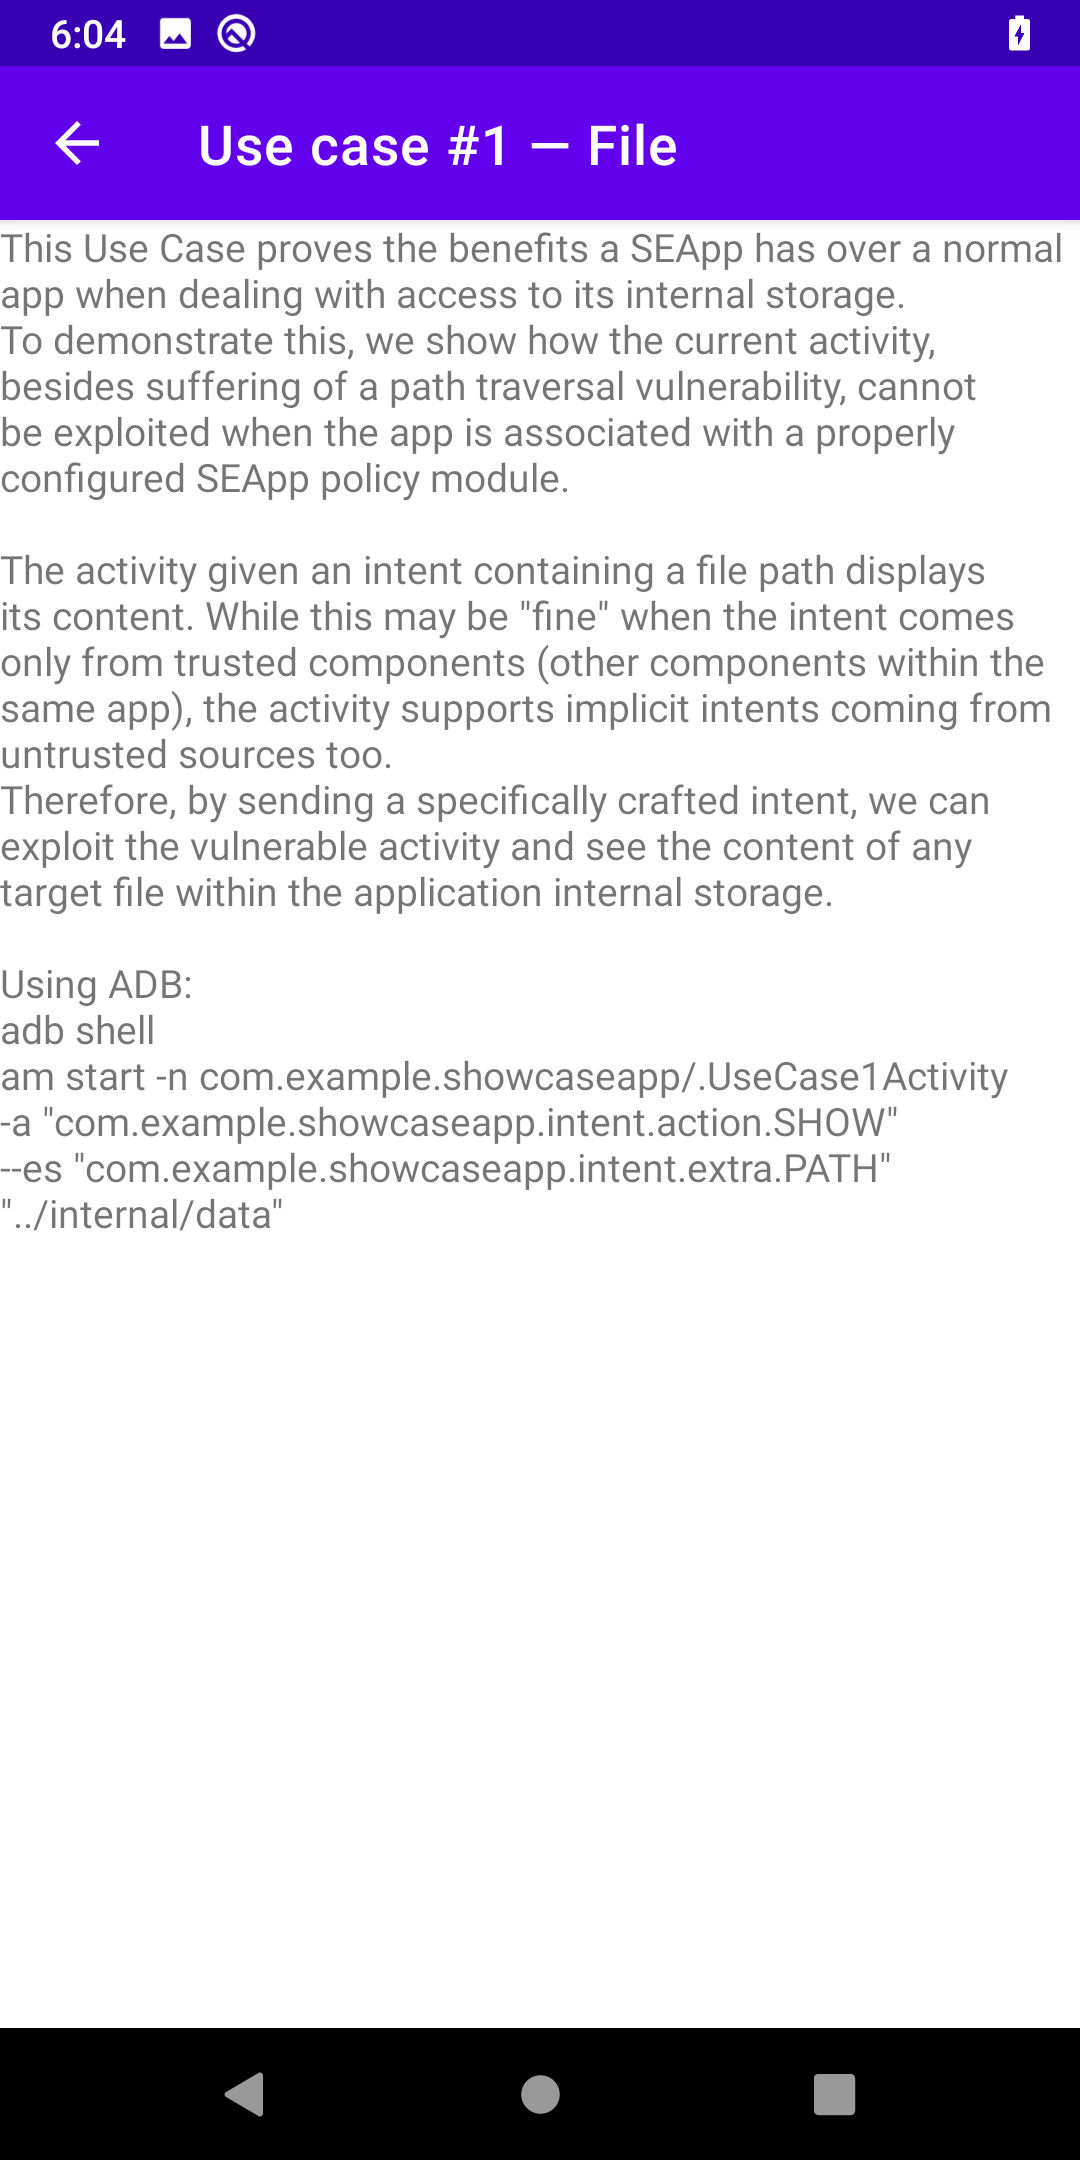
\includegraphics[width=0.28\textwidth]{chapters/seapp/figs/ae/UseCase1Activity.png}}
  \hfill
  \subfloat{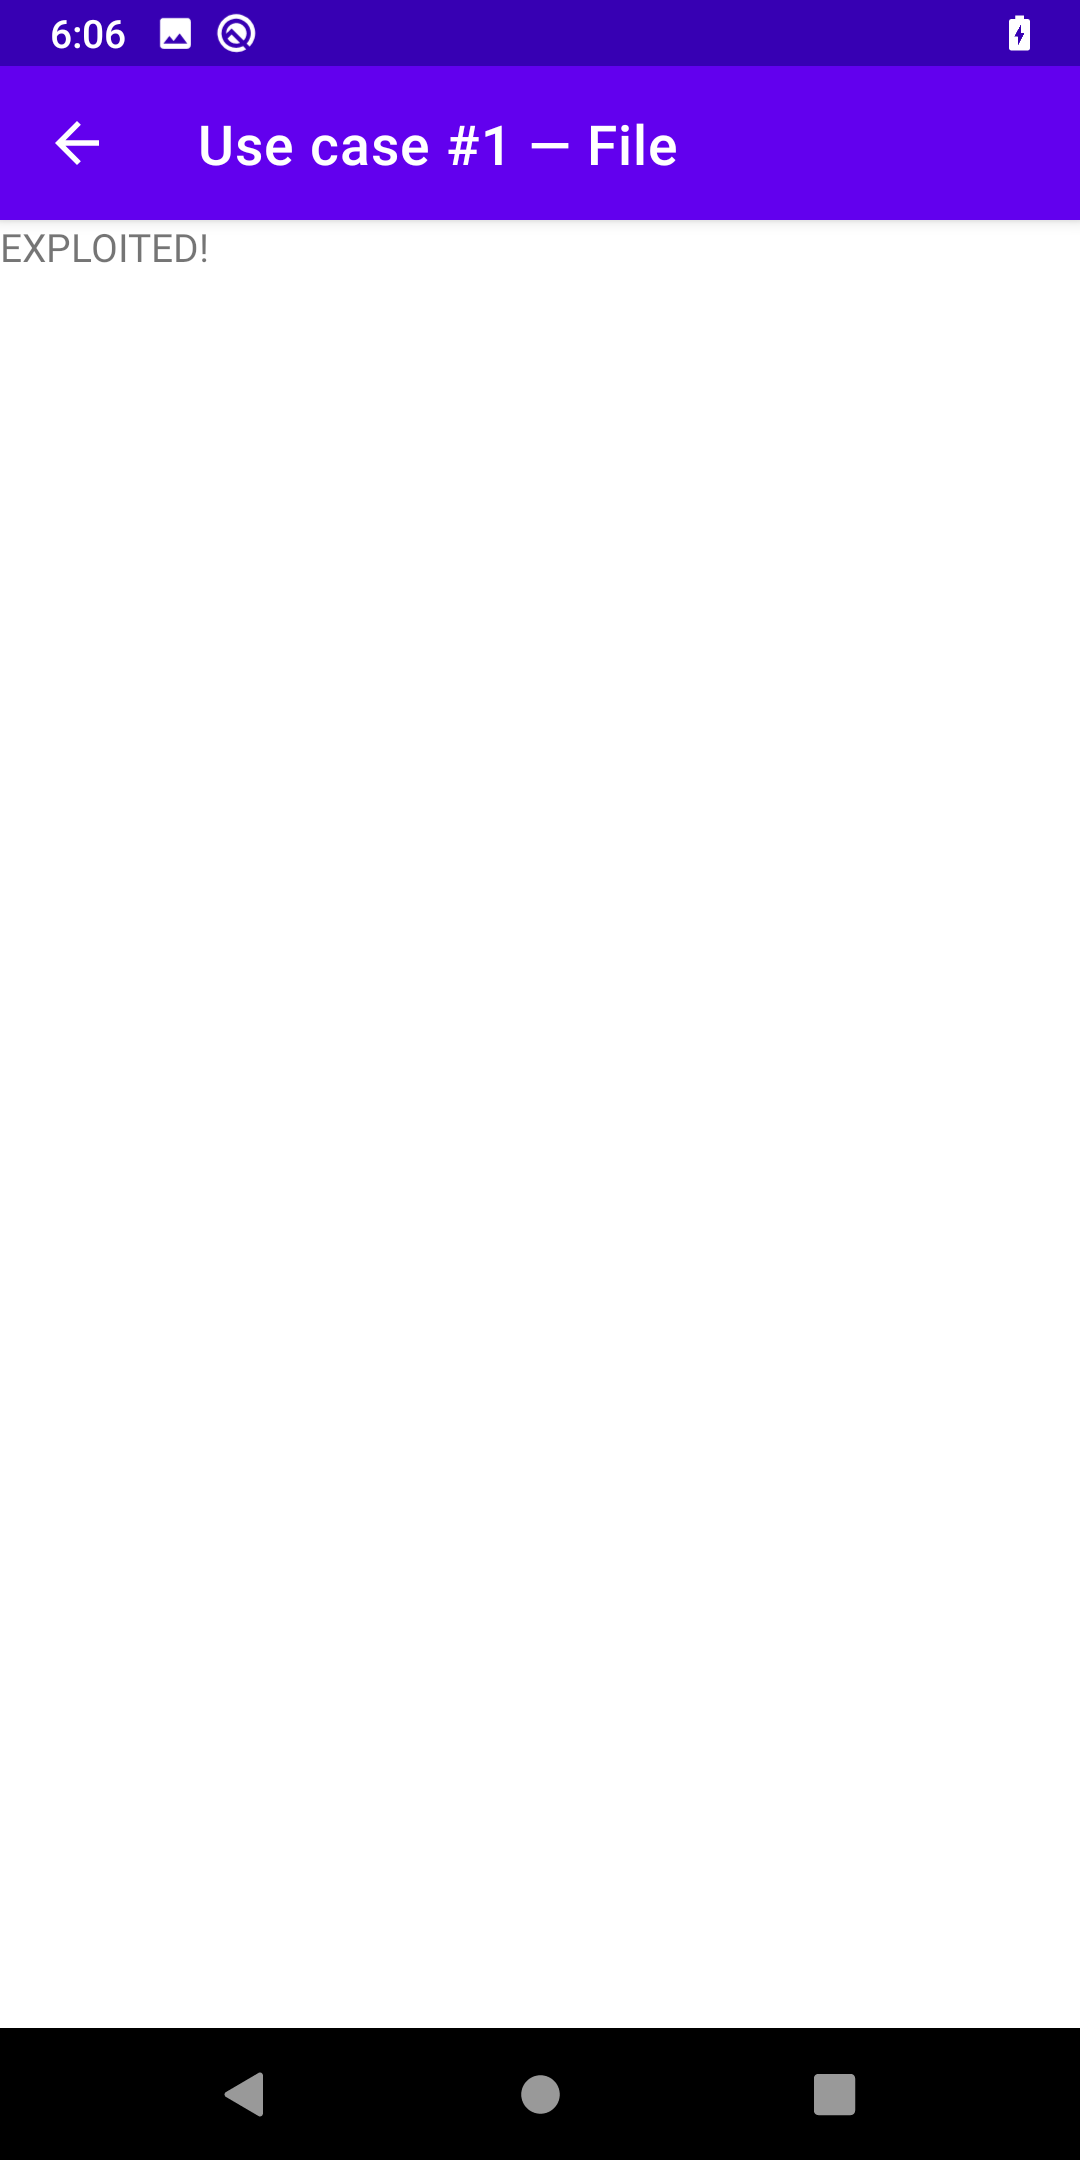
\includegraphics[width=0.28\textwidth]{chapters/seapp/figs/ae/UsaCase1ActivityExploited.png}}
  \hfill
  \subfloat{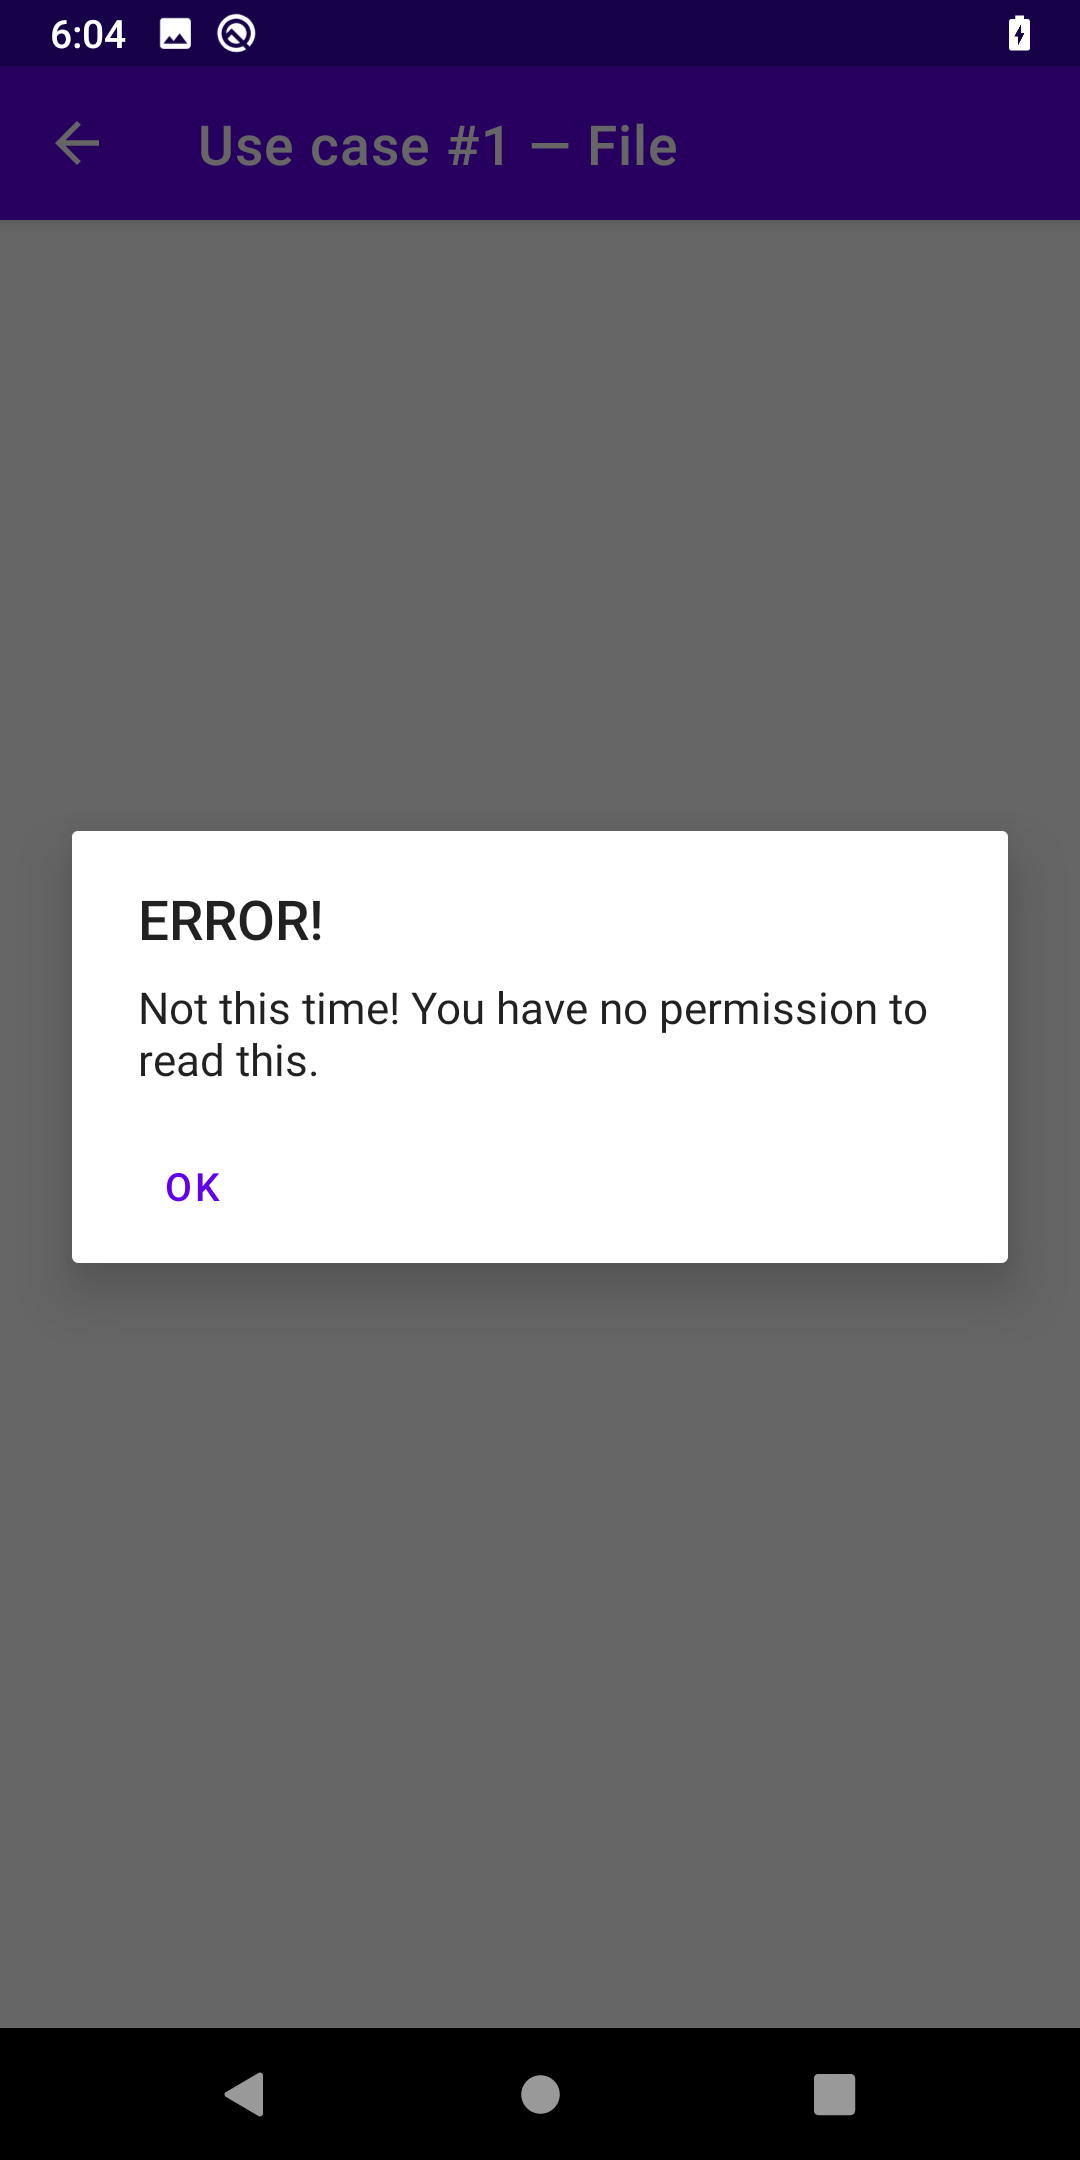
\includegraphics[width=0.28\textwidth]{chapters/seapp/figs/ae/UseCase1ActivityNotExploited.png}}
  \caption{\label{fig:seapp_uc1_views}\bf Use case 1 views}
\end{figure}

\begin{figure}[h!]
  \centering
  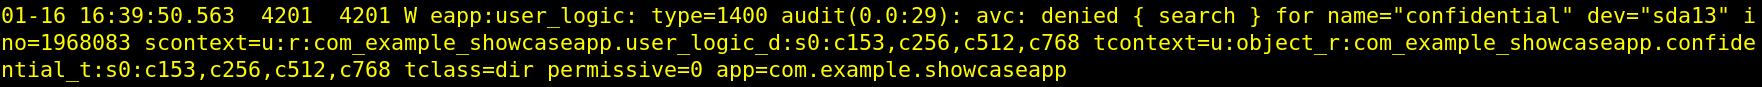
\includegraphics[width=\textwidth]{chapters/seapp/figs/ae/UseCase1Logcat.png}
  \caption{\label{fig:seapp_uc1_logcat}\bf Use case 1 logcat}  
\end{figure}

\newpage
      

%%% Local Variables: 
%%% mode: latex
%%% TeX-master: "../../../../main.tex"
%%% reftex-default-bibliography: "../../../../bib/biblio.bib"
%%% End:

\section{UC\#2: fine-granularity in access to services}\label{appendix:seapp_uc2}

In this use case we show how to confine an Ad library into an ad-hoc
process, with guarantees that it cannot abuse the access privileges
granted to the whole application sandbox by the user.  To do that, we
deliberately inject, in the same process the library is executed, a
malicious component (which is directly invoked by the library) that
tries to capture the location when the permission {\em
  ACCESS\textunderscore FINE\textunderscore LOCATION} is granted to
the app. The Ad library used is Unity Ads~\cite{seapp_unityads}, which
according to~\cite{seapp_ads_use} in 2020 was used by 11\% of apps
that show ads.
%
\begin{figure}[h]
  \centering
  \subfloat{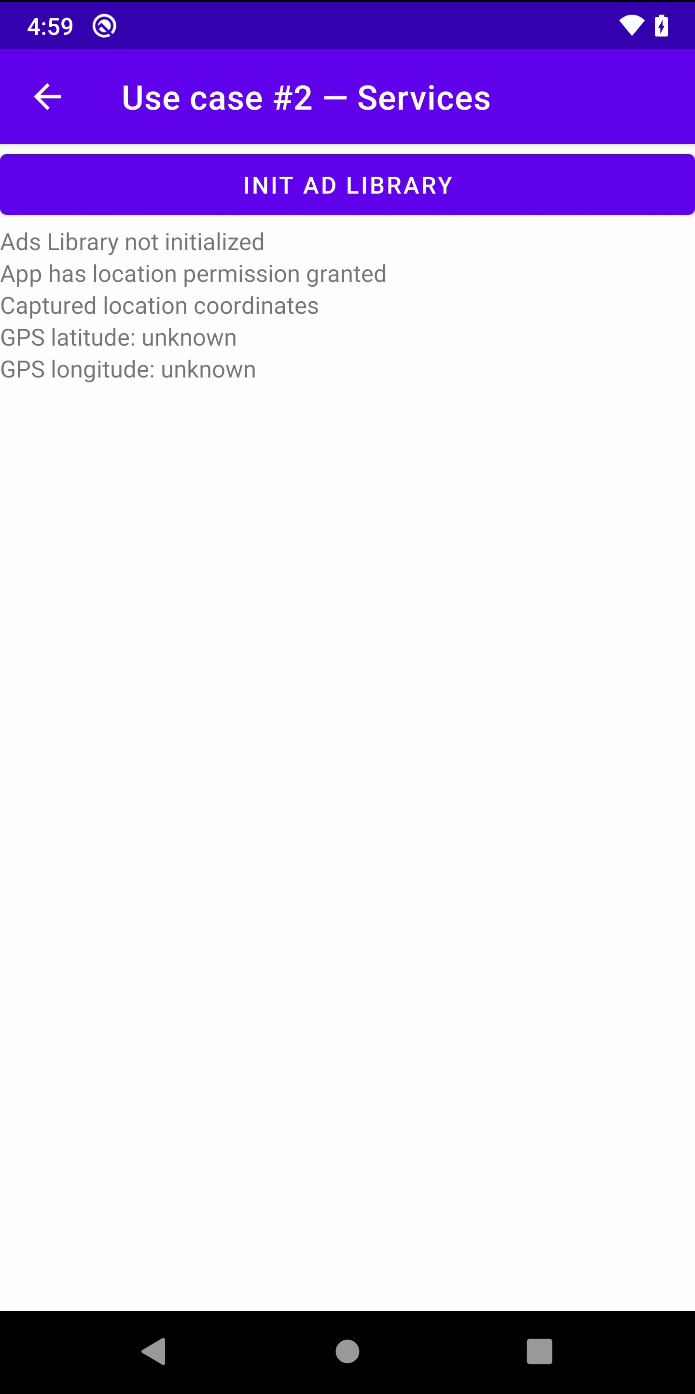
\includegraphics[width=0.3\textwidth]{chapters/seapp/figs/ae/uc21.png}}
  \hfill
  \subfloat{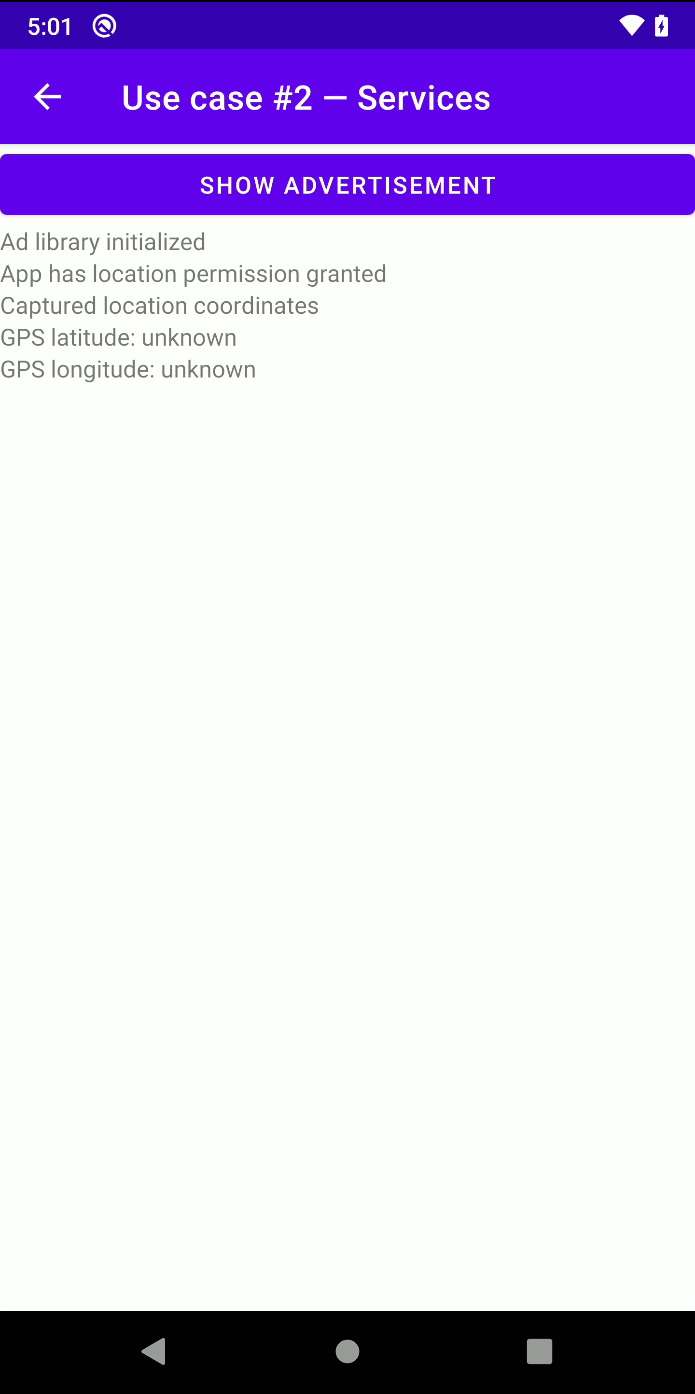
\includegraphics[width=0.3\textwidth]{chapters/seapp/figs/ae/uc22.png}}
  \hfill
  \subfloat{
\includegraphics[width=0.3\textwidth]{chapters/seapp/figs/ae/uc23.png}}
  \caption{\label{fig:seapp_uc2_views} UC\#2 views}
\end{figure}

In this case the library is invoked by {\em UseCase2Activity}
(Figure~\ref{fig:seapp_uc2_views}a), and according to line 3 of the
\seappcontexts, both the activity and the components created by the
library are executed by {\em Zygote} in a process labeled with {\tt
  ads\_d}.  To interact with the Ad library, {\em UseCase2Activity}
instances a {\tt UnityAdsListener}.  After the Ad initialization
(including the registration of the listener) and displaying the Ad to
the user (Figures~\ref{fig:seapp_uc2_views}b-c), the Ad framework
invokes the listener callback method {\tt onUnityAdsFinish}, which
executes the malicious routine {\tt captureLocation}. The routine
probes the app permissions; if {\em ACCESS\textunderscore
  FINE\textunderscore LOCATION} is granted to the app, the malicious
component retrieves through the \servicemanager a handle to the {\tt
  LocationManager}, and registers to it an asynchronous listener to
capture GPS location (Figure~\ref{fig:seapp_uc2_exploit}).

We show that when the policy module is enforced by \seapp, the malicious
component cannot access the GPS coordinates. This is because the
component is executed in the same process of the library, which is
labeled with {\tt ads\textunderscore d}. If we look at the \sepolicy
(lines 43-50), {\tt ads\_d} is not granted access to the \sel type
{\tt location\textunderscore service}, so the malicious routine cannot
retrieve and therefore connect to the {\em location\textunderscore
  service}.  The following denial is written to the system log: {\em
  denied {\tt find} on {\tt location\textunderscore service} to the
  {\tt ads\textunderscore d} domain}
(Figure~\ref{fig:seapp_uc2_logcat1}). As a result, the malicious
component is terminated by the {\em ActivityTaskManager}
(Figure~\ref{fig:seapp_uc2_logcat2}).

The Ad library was included in the app as an {\em .aar}
archive. To confine it, no modification was necessary, only
the use of \manifest and \sepolicy was required.

\begin{figure}[h]
  \centering
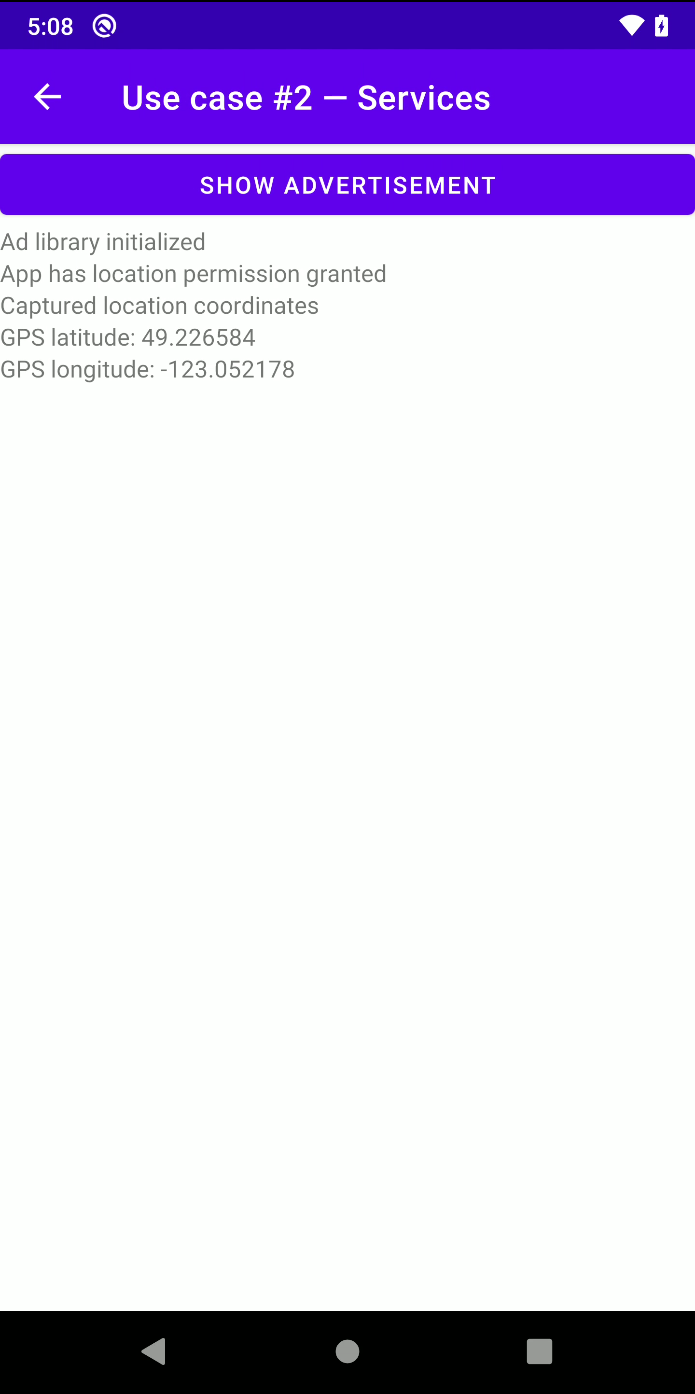
\includegraphics[width=0.29\textwidth]{chapters/seapp/figs/ae/uc24.png}
  \caption{\label{fig:seapp_uc2_exploit} UC\#2 malicious gadjet retrieves location data}
\end{figure}  

\begin{figure}[h]
  \centering
  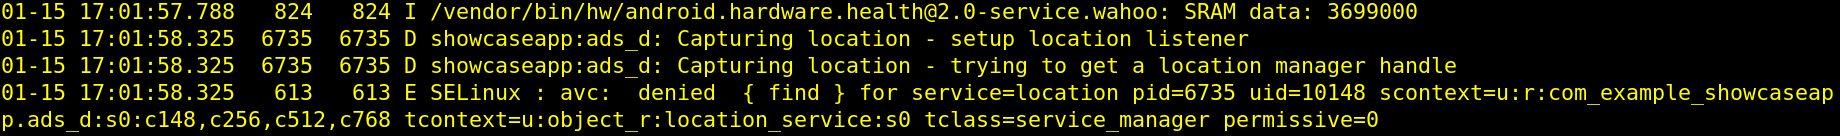
\includegraphics[width=\textwidth]{chapters/seapp/figs/ae/uc25.png}
  \caption{\label{fig:seapp_uc2_logcat1} UC\#2 \sel denial message in the system log}
\end{figure}      

\begin{figure}[h]
  \centering
  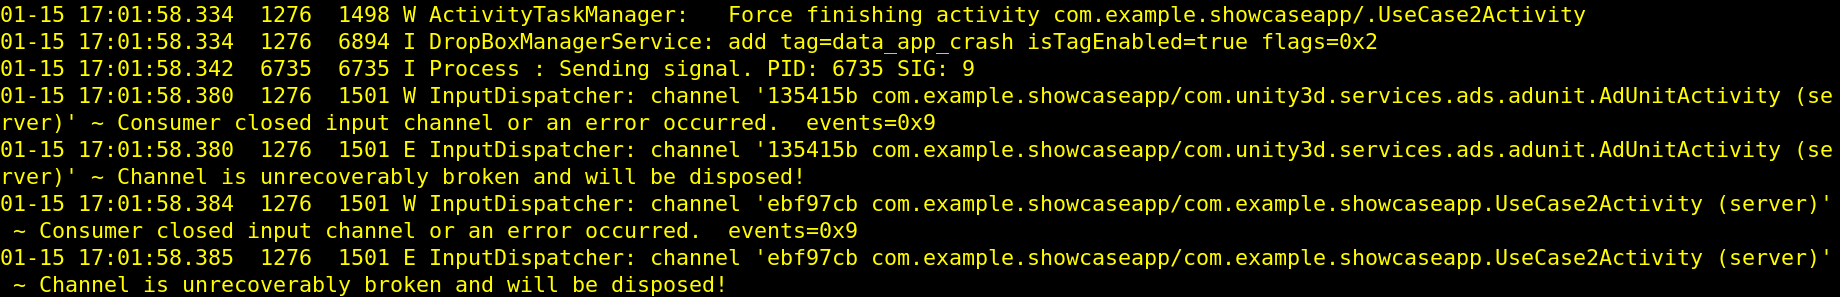
\includegraphics[width=\textwidth]{chapters/seapp/figs/ae/uc26.png}
  \caption{\label{fig:seapp_uc2_logcat2} UC\#2 activity termination due to \sel denial}
\end{figure}      


%%% Local Variables: 
%%% mode: latex
%%% TeX-master: "../../../../main.tex"
%%% reftex-default-bibliography: "../../../../bib/biblio.bib"
%%% End:

\newpage
\section{Use case 3}\label{appendix:seapp_uc3}

In this use case we show how to confine a set of components, which
rely on a high performance native library written in C to perform some
task. Our goal is to demonstrate that the context running the native
library code is prevented to access the network, even when the
permissions {\em INTERNET} and {\em ACCESS\textunderscore
  NETWORK\textunderscore STATE} are granted to the app sandbox.

\begin{figure}[h]
  \centering
  \subfloat{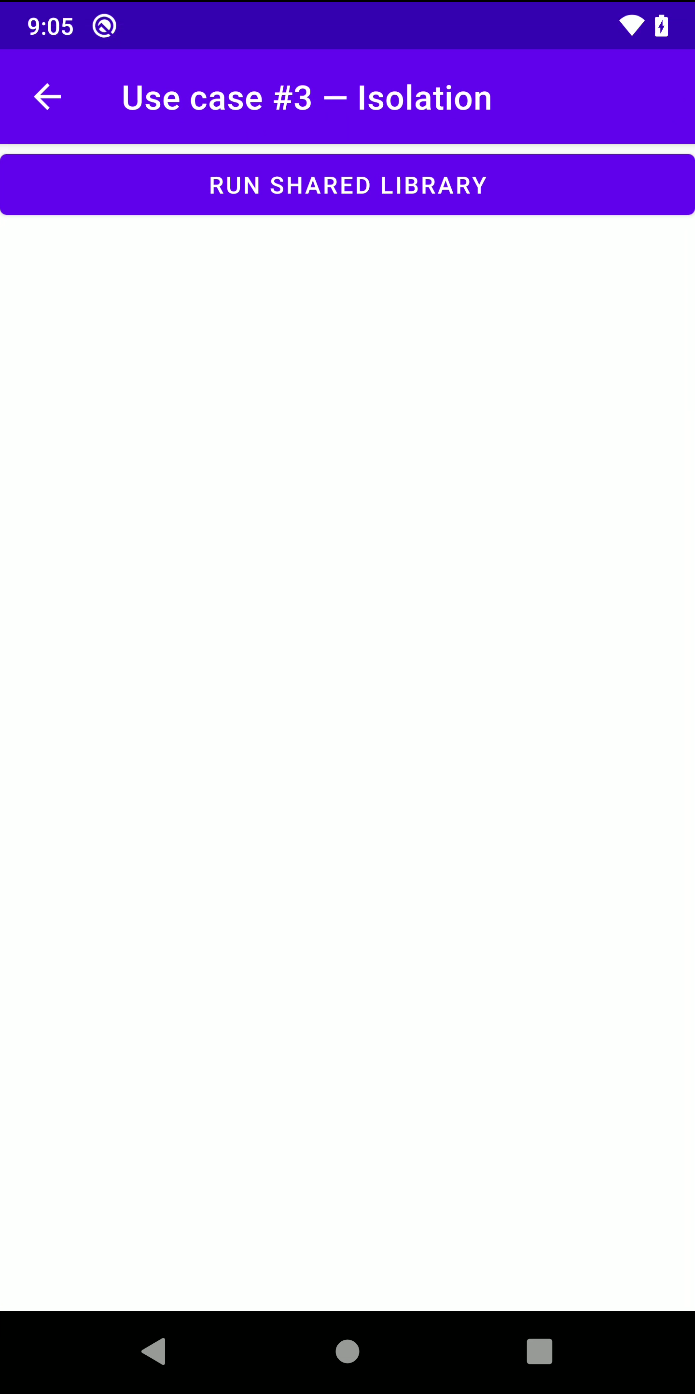
\includegraphics[width=0.3\textwidth]{chapters/seapp/figs/ae/uc31.png}}
  \hfill
  \subfloat{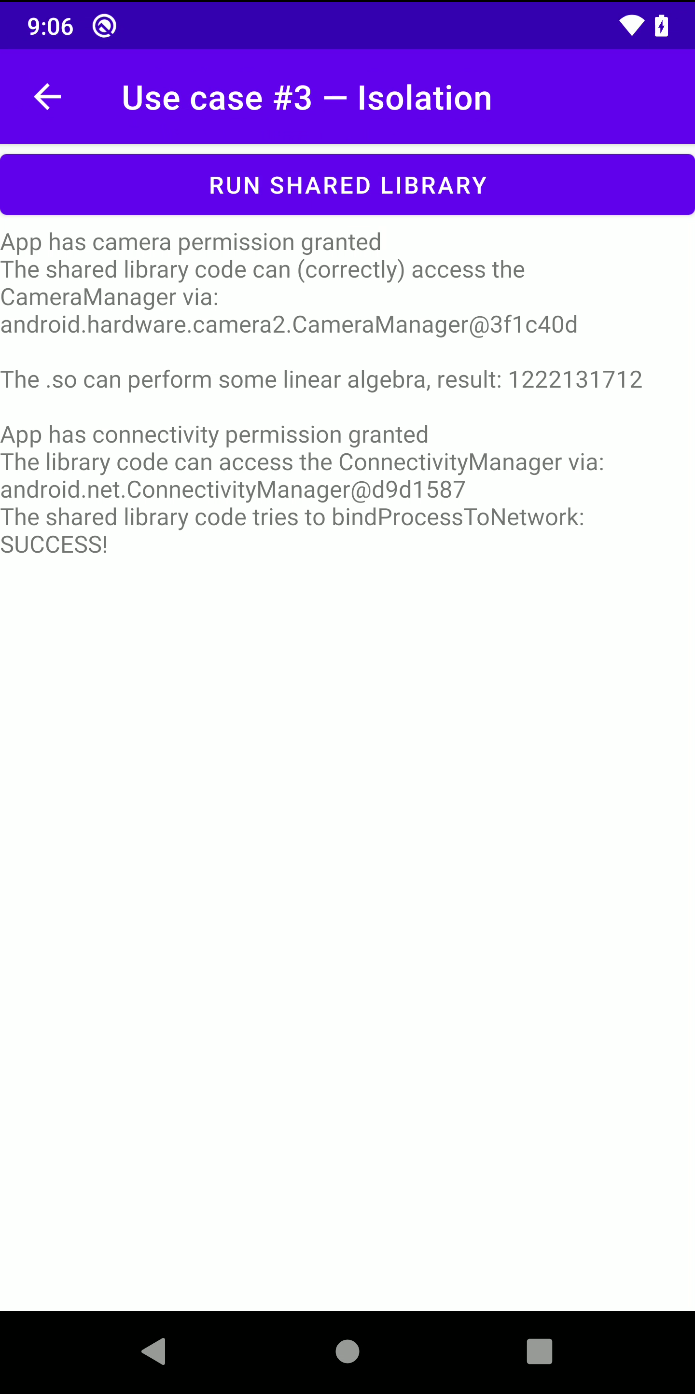
\includegraphics[width=0.3\textwidth]{chapters/seapp/figs/ae/uc32.png}}
  \hfill
  \subfloat{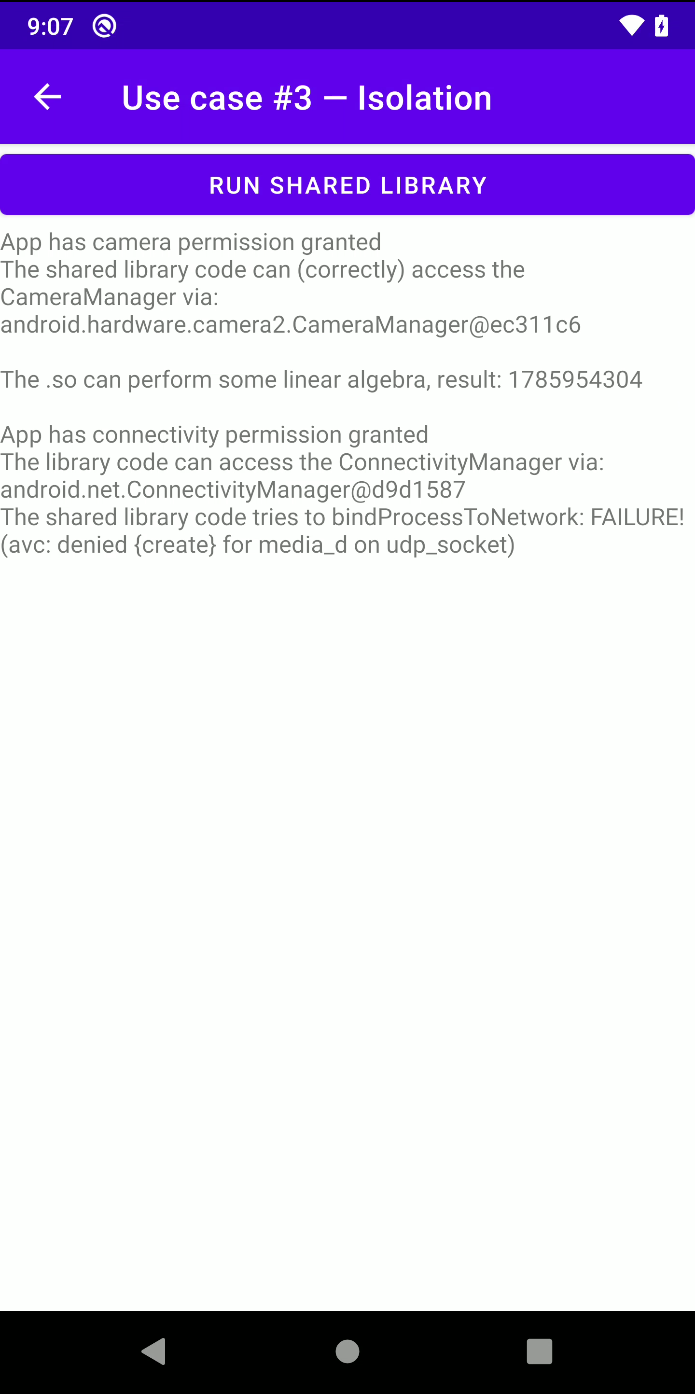
\includegraphics[width=0.3\textwidth]{chapters/seapp/figs/ae/uc33.png}}
  \caption{\label{fig:seapp_uc3_views} Use case 3 views}
\end{figure}

The native library is invoked by {\em UseCase3Activity}
(Figure~\ref{fig:seapp_uc3_views}a), which, according to line 4 in the
\seappcontexts, is executed in a process labeled with {\tt media\_d}
by {\em Zygote}.  The call to the library is performed via JNI. Its
job is to connect to the {\em camera\textunderscore service} and take
a picture.  Since the app is granted the {\em CAMERA} permission, the
native library code (legitimately, line 53 in the \sepolicy) connects
to the {\tt CameraManager}.

Since the native library performs image processing, we do not want it
to access the network. However, the permissions {\em INTERNET} and
{\em ACCESS\textunderscore NETWORK\textunderscore STATE} are granted
to the app, as they are required by the Ads framework.  Thus, when the
policy module is not available, the native library can connect to the
{\tt ConnectivityManager} and successfully bind the current process to
the network (Figure~\ref{fig:seapp_uc3_views}b).  Instead, when the
policy module is enforced by SEApp, since {\tt media\_d} was granted
only the basic app permissions (line 11 in \sepolicy), the connection
to the network is forbidden (Figure~\ref{fig:seapp_uc3_views}c).  This
happens because binding a process to the network is associated with
opening a network socket, an operation not permitted by \sel without
the required permissions. The following denial is written to the
system log: {\em denied {\tt create} on {\tt udp\textunderscore
    socket} to {\tt media\textunderscore d} domain}
(Figure~\ref{fig:seapp_uc3_logcat}).

\begin{figure}[h]
  \centering
  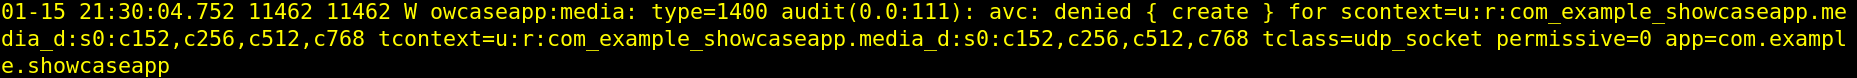
\includegraphics[width=\textwidth]{chapters/seapp/figs/ae/uc35.png}
  \caption{\label{fig:seapp_uc3_logcat} Use case 3 logcat - \sel denial}  
\end{figure}      

This use case, besides showing how SEApp confines a native library,
also demonstrates the power and simplicity of the macro, as adding the
line {\tt (call md\textunderscore netdomain (media\textunderscore d))}
to the policy module grants to {\tt media\textunderscore d} the needed
permissions to access the network.  The application developer is thus
not required to know or understand the internal \sel policy in order
to leverage this functionality.

The isolation properties introduced by \pap applies also to other
common security problems presented
in~\cite{seapp_common_play_protect_vulnerabilites}. Just to mention
one, \pap can mitigate the impact of incorrect sandboxing of a
scripting language.

%%% Local Variables: 
%%% mode: latex
%%% TeX-master: "../../../../main.tex"
%%% reftex-default-bibliography: "../../../../bib/biblio.bib"
%%% End:

\section[Policy module]{Showcase app policy module}\label{appendix:seapp_policy}

Here are reported the showcase app policy module files.
\begin{lstlisting}[
  language=policyfile, caption=Showcase app \seappcontexts,
  numbersep=2pt, resetmargins=false, label=seapp_seappctxp,
  aboveskip=4mm, belowskip=1mm
]
user=_app seinfo=showcase_app domain=com_example_showcaseapp.core_logic_d name=com.example.showcaseapp:core_logic levelFrom=all
user=_app seinfo=showcase_app domain=com_example_showcaseapp.user_logic_d name=com.example.showcaseapp:user_logic levelFrom=all
user=_app seinfo=showcase_app domain=com_example_showcaseapp.ads_d name=com.example.showcaseapp levelFrom=all
user=_app seinfo=showcase_app domain=com_example_showcaseapp.media_d name=com.example.showcaseapp:media levelFrom=all
\end{lstlisting}
\begin{lstlisting}[
  language=policyfile, caption=Showcase app \filecontexts,
  numbersep=2pt,resetmargins=false, label=seapp_filectxp,
  aboveskip=2mm, belowskip=1mm
]
.*                  u:object_r:app_data_file:s0
files/confidential  u:object_r:com_example_showcaseapp.confidential_t:s0
files/ads_cache     u:object_r:com_example_showcaseapp.ads_t:s0
\end{lstlisting}
\begin{lstlisting}[
  language=policyfile, caption=Showcase app \macpermissions,
  numbersep=2pt, resetmargins=false, label=seapp_macctxp,
  aboveskip=2mm, belowskip=1mm
]
<?xml version="1.0" encoding="iso-8859-1"?>
<policy>
  <signer signature="SIGNATURE">
    <package name="com.example.showcaseapp">
      <seinfo value="showcase_app"/>
    </package>
  </signer>
</policy>
\end{lstlisting}
\begin{lstlisting}[
  language=policyfile, caption=Showcase app \sepolicy,
  numbersep=2pt, resetmargins=false, label=seapp_sepolctxp,
  aboveskip=2mm, belowskip=1mm, basicstyle=\footnotesize\ttfamily,
]
(block com_example_showcaseapp
  ; creation of domain types
  (type core_logic_d)
  (call md_untrusteddomain (core_logic_d))
  (type user_logic_d)
  (call md_appdomain (user_logic_d))
  (type ads_d)
  (call md_appdomain (ads_d))
  (call md_netdomain (ads_d))
  (type media_d)
  (call md_appdomain (media_d))
  (typeattribute domains)
  (typeattributeset domains (core_logic_d user_logic_d ads_d media_d))

  ; creation of file types
  (type confidential_t)
  (call mt_appdatafile (confidential_t))
  (type ads_t)
  (call mt_appdatafile (ads_t))

  ; bounding the domains and types
  (typebounds untrusted_app core_logic_d)
  (typebounds untrusted_app user_logic_d)
  (typebounds untrusted_app ads_d)
  (typebounds untrusted_app media_d)	
  (typebounds app_data_file confidential_t)
  (typebounds app_data_file ads_t)

  ; grant core_logic_d access to confidential files
  (allow core_logic_d confidential_t (dir (search write add_name)))
  (allow core_logic_d confidential_t (file (create getattr open read write)))
  ; grant ads_d access to ads_cache files
  (allow ads_d ads_t(dir(search write add_name)))
  (allow ads_d ads_t(file(create getattr open read write)))

  ; minimum app_api_service subset
  (allow domains activity_service (service_manager (find)))
  (allow domains activity_task_service (service_manager (find)))
  (allow domains ashmem_device_service (service_manager (find)))
  (allow domains audio_service (service_manager (find)))
  (allow domains surfaceflinger_service (service_manager (find)))
  (allow domains gpu_service (service_manager (find)))

  ; grant core_logic_d access to the necessary services
  (allow core_logic_d restorecon_service (service_manager (find)))
  (allow core_logic_d location_service (service_manager (find)))

  ; grant ads_d access to unity3ads needed services
  (allow ads_d radio_service (service_manager (find)))
  (allow ads_d webviewupdate_service (service_manager (find)))
  (allow ads_d autofill_service (service_manager (find)))
  (allow ads_d clipboard_service (service_manager (find)))
  (allow ads_d batterystats_service(service_manager (find)))
  (allow ads_d batteryproperties_service (service_manager (find)))
  (allow ads_d audioserver_service (service_manager (find)))
  (allow ads_d mediaserver_service (service_manager (find)))

  ; grant media_d access to the necessary services
  (allow media_d autofill_service (service_manager (find)))
  (allow media_d cameraserver_service (service_manager (find)))
)
\end{lstlisting}


%%% Local Variables: 
%%% mode: latex
%%% TeX-master: "../../../main.tex"
%%% reftex-default-bibliography: "../../../bib/biblio.bib"
%%% End: